% example.tex
\documentclass[dvisvgm]{minimal}

\usepackage{tikz}
\usetikzlibrary {positioning,
                 shapes.geometric}

\begin{document}
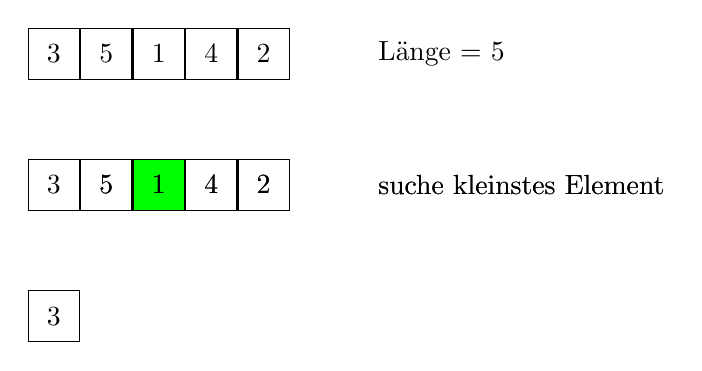
\begin{tikzpicture}[square/.style={regular polygon,regular polygon sides=4}]
    % Grundmuster
    \node[draw, square] (a) {3}; 
    \node[draw, square, right=0cm of a] (b) {5};
    \node[draw, square, right=0cm of b] (c) {1};
    \node[draw, square, right=0cm of c] (d) {4};
    \node[draw, square, right=0cm of d] (e) {2};
    \node[right= of e] (e_text) {Länge = 5};

    % S1.1
    \node[draw, square, below = of a] (a11) {3}; 
    \node[draw, square, right=0cm of a11] (b11) {5};
    \node[fill=green,
          draw, square, right=0cm of b11] (c11) {1};
    \node[draw, square, right=0cm of c11] (d11) {4};
    \node[draw, square, right=0cm of d11] (e11) {2};
    \node[right= of e11] (e11_text) {suche kleinstes Element};

    % S2.1
    \node[draw, square, below = of a11] (a21) {3}; 
    \node[draw, square, right=0cm of a11] (b21) {5};
    \node[draw, square, right=0cm of b11] (c21) {1};
    \node[draw, square, right=0cm of c11] (d21) {4};
    \node[draw, square, right=0cm of d11] (e21) {2};
    \node[right= of e21] (e21_text) {suche kleinstes Element};

\end{tikzpicture}
\end{document}